\documentclass{article}

\usepackage{url} % Tidy web links
\usepackage{microtype} % 'Improved' typesetting
\usepackage{parskip} % Adds white space between paragraphs
\usepackage[super]{natbib} % Citations using superscript
\usepackage[a4paper, left=2.cm, right=2.0cm, top=2.0cm, bottom=2.0cm]{geometry}
\usepackage{longtable,booktabs}  % For tables
\usepackage{caption} % For figure and table captions
\usepackage{graphicx} % Adds more functionality to graphics for inclusion of figures
\usepackage{lineno} % Allows use of \linenumbers to add line numbers 
\usepackage[toc,page]{appendix}
\usepackage[utf8]{inputenc}
\frenchspacing % No double spacing between sentences
\linespread{1.2} % Set linespace
\usepackage{authblk} % For author formatting
\usepackage{lmodern} % A scalable font - avoids erros due to non-sclabale fonts
\usepackage{subcaption} % Allows use of subfigures
\DeclareUnicodeCharacter{2060}{\nolinebreak} % Prevent unicode (U+2060) error on local complile
\usepackage{cclicenses} % For creative commons license
\usepackage{xcolor} % for coloured text
\usepackage{xurl} %for url but with more flexible linebreaking

\usepackage{markdown}

% Choose your own colour
\usepackage{color}
\newcommand{\mjanote}[2][\textcolor{red}{\dagger}]{\textcolor{red}{$#1$}\marginpar{\color{red}\raggedright\tiny$#1$ #2}}
\newcommand{\mjaFIXME}[1]{\textcolor{red}{[\textbf{FIXME} \textsl{#1}]}}
\newcommand{\kpnote}[2][\textcolor{magenta}{\dagger}]{\textcolor{magenta}{$#1$}\marginpar{\color{magenta}\raggedright\tiny$#1$ #2}}
\newcommand{\kpFIXME}[1]{\textcolor{magenta}{[\textbf{FIXME} \textsl{#1}]}}

\hbadness=1000000 % Turn off \hbox badness warnings

\renewcommand{\thefootnote}{\textit{\alph{footnote}}} % Lettered footnotes

% Word counts
\usepackage{verbatim}

\newcommand{\detailtexcount}[1]{%
  \immediate\write18{texcount -sub=section -merge -sum -q #1.tex output.bbl > #1.wcdetail }%
  \verbatiminput{#1.wcdetail}%
}

\newcommand{\quickwordcount}[1]{%
  \immediate\write18{texcount -1 -sum -merge -q #1.tex output.bbl > #1-words.sum }%
  \input{#1-words.sum} words%
}

%\newcommand{\quickcharcount}[1]{%
%  \immediate\write18{texcount -1 -sum -merge -char -q #1.tex output.bbl > #1-chars.sum }%
%  \input{#1-chars.sum} characters (not including spaces)%
%}

\newcommand{\charactercount}[1]{
\immediate\write18{
    expr `texcount -1 -sum -merge #1.tex` + `texcount -1 -sum -merge -char #1.tex` - 1 
    > chars.txt
}\input{chars.txt} characters (inc spaces)}

\begin{document}
% Rewrite this title to include dementia

\title{STROKE-FLOW: Using explainable machine learning and clinical pathway simulation to model and optimise flow and capacity planning in the in-patient stroke pathway.}

\author{} % Hide author
\date{} % Hide date
\maketitle
\vspace{-20mm}
%\section{Summary}

The focus of our work is on using explainable machine learning and clinical pathway simulation, applied to national clinical audit data to identify between-hospital variation in clinical decision-making, and understanding the impact of that variation on patients and the health service. Our work is in collaboration with the Sentinel National Stroke Audit Programme, and focuses mostly on the emergency stroke pathway, and variation in use of clot-busting drugs (the primary treatment of emergency stroke admissions), but is applicable across other clinical areas.

In the proposed project we would like to bring multiple NIHR project strands together in a single framework, and progress the modelling to include acute and rehab in-patient care. As a result we will be able to evaluate how variation in clinical decision-making and processes effect both the patient and bed requirements for in-patient stroke care. This will allow planners to see how an optimal system may behave in their area (e.g. at the level of integrated stroke delivery teams, or integrated care systems). Analysis and modelling will be made available through a web application.

The project will be a multi-methods study including machine learning, clinical pathway simulation, geographic modelling, and qualitative research. The team has the necessary skills and experience, with a well-established track-record, to undertake this work.

\subsection{Process flow in scope}

The work will focus on out-of-hospital stroke patients who call for an ambulance, the system in scope is shown in figure \ref{fig:flow}.

\begin{figure}[h]
\centering
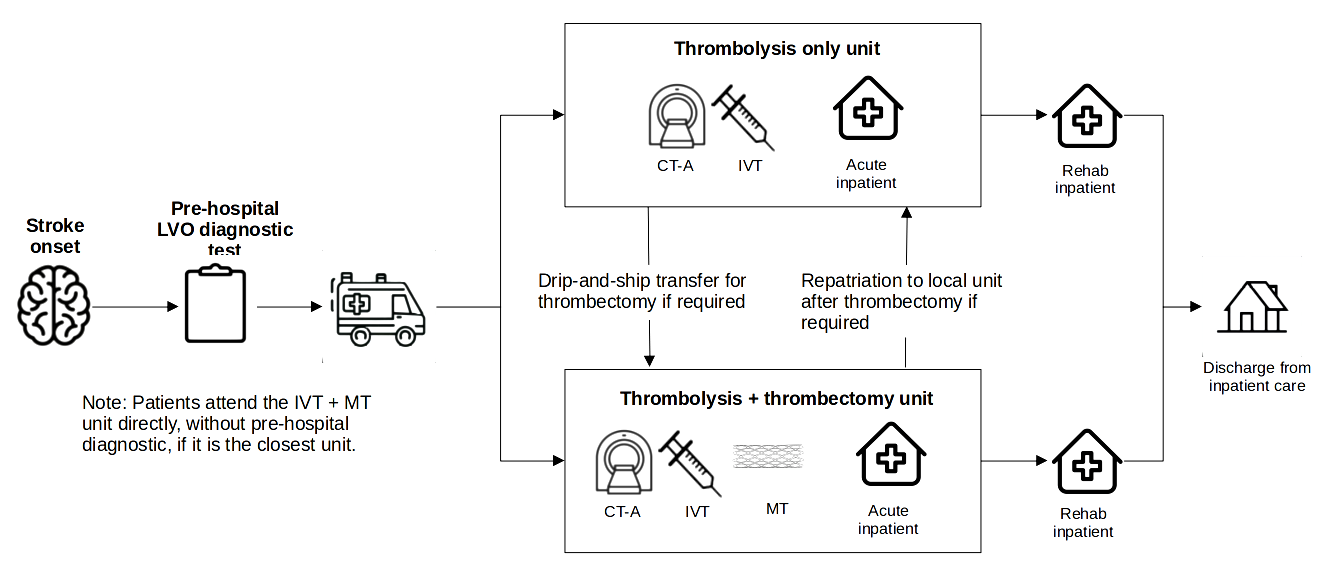
\includegraphics[width=1.0\textwidth]{./images/pathway}
\caption{Summary of patient flow}
\label{fig:flow}
\end{figure}


\subsection{Research questions}

\begin{markdown}
* How much of the variation in required stroke inpatient resources comes from differences in local patient populations, and how much from differences in variation in clinical decision-making and processes?
* How would optimal provision of thrombolysis and thrombectomy (including decision-making on selecting suitable patients) affect outcomes and required stroke inpatient resources?
* How would pre-hospital triage for patients suitable for thrombectomy affect outcomes and required stroke inpatient resources?
* What are hospitals with good outcomes and shorter lengths of stay (after allowing for differences in local populations) doing differently, compared with those with longer lengths of stay?
\end{markdown}


%\section{Bid info}

\url{https://www.nihr.ac.uk/funding/2310-health-and-social-care-delivery-research-programme-researcher-led/32515}

\subsection{Timelines}

\begin{markdown}
* Stage 1 deadline: 1pm, 20 September 2023
* Notification of out of remit/non-competitive decision if unsuccessful: late October 2023
* Notification of Stage 1 shortlisting decision: early December 2023
* Stage 2 writing window: early December 2023 to early February 2024
* Notification of Stage 2 funding decision: early April 2024
* Start date for funded studies: 1 August/September 2024
\end{markdown}
\section{Research plan}

\vspace{2mm}
\hrule
\textit{`Much of the variation in healthcare is accounted for by the willingness and ability of doctors to offer treatment rather than differences in illness or patient preference'} John Wennberg, the pioneer of research into clinical variation and founder of the Dartmouth Atlas of Health Care.
\vspace{2mm}
\hrule

\subsection{What is the problem?}

Stroke remains one of the leading causes of death and disability, globally and in the UK. The majority of strokes are caused by a clot. Clots may be reduced or removed with \textit{reperfusion} treatments if given soon enough after a stroke. These treatments include thrombolysis, a clot-busting medication given by injection/infusion \cite{emberson_effect_2014} and, more recently, thrombectomy, mechanical removal of a clot performed in a specialist centre \cite{fransen_time_2016}.

Despite thrombolysis being long-established and of proven benefit in ischaemic stroke, use of thrombolysis varies significantly both between hospitals. In England and Wales the national stroke audit reported that in 2021/22, thrombolysis rates for emergency stroke admissions varied from just 1\% to 28\% between hospitals \cite{sentinel_national_stroke_audit_programme_ssnap_2022}, with a median rate of 10.4\%, against a NHS England long term plan that 20\% of patients of emergency stroke admissions should be receiving thrombolysis. Additionally, in 2022/23, 3.2\% of patients received thrombectomy, significantly below the expected eligibility of at least 10\% \cite{mcmeekin_updating_2021}. 

In addition to variation in outcomes due to variation in treatment of patients, there is potential that this variation leads to variation in required NHS resources, as worsened outcomes due to poorer use of thrombolysis or thrombectomy may increase downstream healthcare needs.

Our research team uses various modelling techniques, including \textit{explainable machine learning} and \textit{clinical pathway simulation} to identify the variation that occurs across different hospitals during the first few hours of stroke care. We use these models to understand the the source and impact of that variation on patients \cite{allen_using_2022, allen_use_2022}, identifying the variation that comes from hospitals and processes, rather than variation in local patient populations. We have identified that the majority of between-hospital variation in thrombolysis use comes from differences in hospital processes and decision-making, rather than from differences in local patient populations \cite{allen_using_2022, allen_use_2022}.

We are working with the Sentinel Stroke National Audit Programme and NHS-England on reducing between hospital-variation in emergency stroke care. In this proposed project we will build on previous and existing work, bringing it together into a single analysis framework and web application, and extending work to cover looking at variation in inpatient lengths of stay (and how they are effected by reperfusion treatment), and an explainable machine learning analysis in variation in selection of patients for thrombectomy.

\subsubsection{Relevant prior and current work}

\begin{itemize}
    \item \textbf{Geographical analysis} - analysis of variation in access to thrombolysis and thrombectomy \cite{allen_maximising_2019}.

    \item \textbf{Thrombolysis pathway and variation in patient selection} - analysis of between-hospital variation in the thrombolysis pathway using clinical pathway simulation and explainable machine learning \cite{allen_use_2022, pearn_what_2023}. Current work, as part of the NIHR SAMueL-2 project \footnote{\url{https://fundingawards.nihr.ac.uk/award/NIHR134326}} is focussing on an analysis of how between-hospital variation in selection of patients for thrombolysis effects patient outcomes. This work has produced a web tool \footnote{\url{https://stroke-predictions.streamlit.app/}}, including a health economics model, that is going in to use with the national stroke audit and NHS-England to help facilitate improvement in thrombolysis use, by working with lower thrombolysing units.

    \item \textbf{Pre-hospital pathway} - As part of the NIHR OptImIST programme \footnote{\url{https://fundingawards.nihr.ac.uk/award/NIHR202361}}, we are modelling the effect of pre-hopsital selection of patients for thrombectomy, the effect this is likely to have on time to thrombolysis and thrombectomy, and their outcomes (using a mathematical outcome model based on time to treatment).
    
\end{itemize}

\subsubsection{Proposed work}

See \textit{research questions and aims} below for more details. 

\begin{itemize}
    \item Analysis of variation in patient selection for thrombectomy (and resulting patient outcomes).

    \item Analysis of how variation in use of thrombolysis and thrombectomy effects in-patient length of stay

    \item Causal inference studies on the links between treatment and outcome

    \item Production of a combined analytical pathway and web tool
    
\end{itemize}

\subsection{Why is this work important?}

Reperfusion treatment is the mainstay emergency treatment for stroke. Unwanted variation in reperfusion treatment leads to avoidable variation in disability outcomes in stroke, which also has potential to cause unnecessary variation in downstream healthcare resource use. These methods are also potentially valuable in other healthcare settings where it is suspected that variation in healthcare and outcomes is due to variation in treatment processes and decisions rather than in differences in local patient populations.

\subsection{Review of existing evidence}

Studies have shown that reasons for low and varying thrombolysis rates are multi-factorial. Reasons may often be organisational \cite{aguiar_de_sousa_access_2019, kamal_delays_2017, carter-jones_stroke_2011}. For many organisational factors, the establishment of primary stroke centres has been suggested to improve the emergency care of patients with stroke and reduce barriers to thrombolysis \cite{carter-jones_stroke_2011},  with a centralised model of primary stroke centres leading to increased likelihood of thrombolysis \cite{lahr_proportion_2012, morris_impact_2014, hunter_impact_2013}. 

In addition to organisational factors, clinicians can have varying attitudes on which patients are suitable candidates for thrombolysis. In a discrete choice experiment \cite{de_brun_factors_2018}, 138 clinicians considered hypothetical patient vignettes, and responded as to whether they would give the patients thrombolysis. The authors concluded that there was considerable heterogeneity among respondents in their thrombolysis decision-making. 

Based on national audit data we have previously built models of the emergency stroke pathway using clinical pathway simulation to examine the potential scale of the effect of changing two aspects of the stroke pathway performance (1. the in-hospital process speeds, and 2. the proportion of patients with a determined stroke onset time), and using machine learning to examine the effect of replicating clinical decision-making around thrombolysis from higher thrombolysing hospitals to lower thrombolysing hospitals \cite{allen_using_2022, allen_use_2022}. Using these models we found that it would be credible to target an increase in average thrombolysis in England and Wales, from 11\% to 18\%, but that each hospital should have its own target, reflecting differences in local populations. We found that the largest increase in thrombolysis use would come from replicating thrombolysis decision-making practice from higher to lower thrombolysing hospitals. Two other important factors influencing thrombolysis rates were determination of stroke onset time in some hospitals, and improving the speed of the in-hospital thrombolysis pathway.

We have extended the model to including explainability \cite{pearn_what_2023}. This revealed that lower thrombolysing hospitals, compared with higher thrombolysing hospitals, were particularly less likely to give thrombolysis to patients with 1) mild stroke, 2) imprecisely known onset time, 3) patient with prior disability, 4) any combination of those. This work is now forming the basis of a web tool \footnote{\url{https://stroke-predictions.streamlit.app/}} that allows stroke teams to compare their thrombolysis decisions to others, and to see how changing the pathway process can change the use and speed of thrombolysis, and the effect on patient outcomes.

\subsection{Research questions and aims}

We wish to extend our current work in the following ways:

\begin{itemize}
    \item \textbf{Analysis of variation in patient selection for thrombectomy} - how do thrombectomy centres vary in their selection of patients for thrombectomy, and what is the likely effect on outcomes from this variation?

    \item \textbf{Analysis of how variation in use of thrombolysis and thrombectomy effects in-patient length of stay} - how do thrombolysis and thrombectomy affect length of stay in acute and rehabilitation units?

    \item \textbf{Causal inference studies} - are observations from predictive models supported by causal inference studies, testing that any predictions made can be attributed to the assumed cause.

    \item \textbf{Production of a combined analytical pathway and web tool} - this tool with provide a national and regional analysis of current thrombolysis and thrombectomy use and provision, and enable an analysis of what an optimal system may look like, and the effect that would have on patients and health services. The tool will be developed and refined with co-production workshops, as we work with stroke teams on local thrombolysis and thrombectomy improvement. The web tool will combine:
    
    \begin{enumerate}
        \item Geographical analysis access to thrombolysis and thrombectomy. The map will identify which destination hospital would provide most likely best outcomes depending on type of stroke (of if stroke type is unknown)

        \item Clinical pathway simulation (including the pre-hospital pathway) - showing how optimisation of the pathway may effect thrombolysis and thrombectomy use and speed.

        \item Explainable machine-learning analysis of variation in choice of patients for thrombolysis and thrombectomy (with causal inference methodology to give further confidence in modelling).

        \item A health economics model based on patient outcomes, extending patient outcome results to expected QALY (quality-adjusted life years).
    \end{enumerate} 
    
\end{itemize}

\subsection{Project Plan}

\subsubsection{Data}

We use anonymous patient-level data from the Sentinel Stroke National Audit Programme (SSNAP, \url{https://www.strokeaudit.org/}. SSNAP collects data on essentially all emergency stroke units, from all stroke units in England, Wales, and Northern Ireland. The data includes a wide range of information such as data on times throughout the stroke pathway from stroke onset, pre-stroke disability (modified Rankin Scale, mRS), a breakdown of stroke symptoms using the NIHSS stroke scale, reperfusion treatment given (and timing), comorbidities, death in hospital, disability at discharge from inpatient care, and 6 month follow-up disability (the latter is complete for about 35\% of discharged patients). Data is collected for about 85,000 patients each year, 10-11\% of whom receive thrombolysis, and about 3\% now receiving thrombectomy.

\subsubsection{Design}

The methods used in this study have been used extensively by the team before, except where noted before (the additional of causal inference methodology to strengthen conclusions drawn from observational data). All work will be performed in Python using established libraries for each of the methods. Work will be conducted in \textit{Jupyter notebooks}, all of which will be published in an online \textit{Jupyter Book} as we do for all our work (e.g. see \url{https://samuel-book.github.io/samuel_shap_paper_1/}.

The major components of the project, with methods are as follows:

\begin{itemize}

    \item \textbf{Clinical Pathway Simulation}: We use Clinical Pathway Simulation to model the flow of individual patients through the stroke pathway, with each patient having their own times drawn from distributions (created from observed data), and patient characteristics (e.g. age, stroke severity). Outcome is predicted based on time to treatment for thrombolysis and/or thrombectomy (or based on no treatment given). This model may be used to estimate the effects of changing process speed and efficiency, percentage of patients with ascertained stroke onset time, the likelihood any patient will receive thrombolysis at any hospital, and the choice of which type of hospital to which the patient is conveyed. These models may either be coded in \textit{NumPy} for national scale models, or \textit{SimPy} for regional models where more control is desired over patient flow. We are experienced in both of these methods \cite{allen_use_2022, allen_simulation_2020}

    \item \textbf{Explainable Machine Learning}: We will use machine learning in a range of activities:

    \begin{itemize}
        \item \textit{Learning and and prediction of treatment decisions at different hospitals}. This allows us to learn general patterns of what makes patients suitable for thrombolysis in practice, and allows us to observe how any individual hospital differs from that norm. It also allows us to provide a \textit{benchmark decision} for each patient based upon the majority vote of predicted thrombolysis decisions from a selected group of hospitals. 

        \item \textit{Learning and and prediction of outcomes with and without treatment}. Learning outcomes from observational data extends our mathematical models based on clinical trial results, and allows more complex learning than available from clinical trials. All patients in the data set have estimated disability score prior to stroke, and disability on discharge assessed. We currently predict outcomes with and without thrombolysis, and will extend this to thrombectomy.

        \item \textit{Learning and and prediction of inpatient lengths of stay and discharge destination.} We will extend out machine learning to predict inpatient lengths of stay and discharge destination based on patient details, treatment, and hospital attended. This will allow us to evaluate how thrombolysis and thrombectomy affect lengths of stay and discharge destination independent of patient characteristics, and allow us to investigate any variation in length-of-stay that are attributable to the hospital (which will also me matched to outcomes as a counter-measure of length of stay).
        
    \end{itemize}

    We have tested a range of machine learning models (from logistic regression through to modular neural networks) \cite{allen_using_2022}, but now focus on using \textit{XGBoost}. We add an explainable machine learning model, using \textit{SHAP}, to show how patient features influence the model's predictions. This is done at both patient and population level \cite{pearn_what_2023}.  

    \item \textbf{Causal Inference}: Causal inference will be used to further test whether predictions from the machine learning model are likely to be causal in nature. For example, some patterns are appearing in our current work which may help guide clinicians on use of thrombolysis. In mild stroke (which was not generally included in the clinical trials), we observe that early thrombolysis is associated with a reduced chance of death, whereas later thrombolysis is associated with an increased chance of death. It is possible, however, that this effect is co-incidental rather than causal. We will add established causal inference methods to further test these relationships. We will focus on two key methods:

    \begin{itemize}
        \item Use of \textit{`Propensity'}, the likelihood of a person receiving thrombolysis (estimated from a separate machine learning model). This may be used to stratify or weight results by suitability for treatment, or may be added to outcome models, allowing the outcome model to be adjusted for patients' suitability for treatment. Microsoft have brought together a range of causal inference methods in two Python libraries, \textit{DoWhy} and \textit{EconML}, which we will use for this work.

        \item Use of \textit{Directed Acyclic Graphs} (DAGs). DAGs are simple diagrams showing proposed or assumed causal influences. They are easily understood by non-technical audiences, and so form an excellent basis for discussions and workshops to explore proposed causal relationships with clinical experts. We will use these, alongside results from other methods, in co-production workshops.
    \end{itemize}

    \item 

    \item \textbf{Geographic modelling}: Geographic modelling is used to estimate travel times to closest thrombolysis and thrombectomy units, as well as the travel time between the two types of units when a secondary transfer is required. This type of modelling helps planners understand the likely impact of changes to configurations of health services. We use the Linux \textit{routino} application with \textit{Open Street Map} data for estimating travel times from all Lower Super Output areas to all thrombolysis and thrombectomy units (results are calibrated against Google maps). Mapping is performed using the Python \textit{Geopandas} library.

    \item \textbf{Health economics}: Prof McMeekin has developed a Health Economics model for stroke based on age, sex, and disability at discharge. We already make this model available in our pilot web application (\url{https://stroke-predictions.streamlit.app/Lifetime_mortality}, and it is being written up for publication. As the model is based on disability at discharge we are able to use the same model in the proposed work that also includes thrombectomy as our modelling will estimate disability at discharge under varying scenarios.

    \item \textbf{Web application}: We have a pilot web application (\url{https://stroke-predictions.streamlit.app/}. We use Python-based \textit{StreamLit} which enables data scientists to readily build and maintain web applications.
    
\end{itemize}


\subsubsection{Project team}

The project teams bring together experience of stroke care, machine learning, epidemiology, clinical trials, and causal inference work.

\begin{itemize}

    \item \textbf{Michael Allen (Co-PI, 35\% FTE)} co-leads our NIHR funded work on explainable machine learning \footnote{https://fundingawards.nihr.ac.uk/award/NIHR134326}, with a focus on the technical aspects of the project. Dr Allen has extensive experience of health systems modelling and machine learning.

    \item \textbf{Martin James (Co-I, 5\% FTE)} is a stroke consultant and clinical director of the national stroke audit. Prof James co-leads our NIHR funded work on explainable machine learning \footnote{https://fundingawards.nihr.ac.uk/award/NIHR134326}, with a focus on clinical oversight of the project. Prof James will provide clinical leadership and oversight for this proposed project.

    \item \textbf{Kerry Pearn (Co-PI, 35\% FTE)} has been the principal developer of our explainable machine learning methodology for prediction of thrombolysis use and outcome. Ms Pearn will be responsible for leading the machine learnign aspect of this work, and will contribute to the coding of that work.

    \item \textbf{Peter McMeekin (Co-I, 10\% FTE)} is health economist specialising in stroke care. Prof McMeekin has been responsible for our long term QALY and cost predictions for our previous work, and will continue to lead the health economics aspects of this work.

    \item \textbf{Richard Everson (Co-I, 5\% FTE)} is professor of Machine Learning at the University of Exeter, and has a very broad experience of computer sceince methods. Prof Everson will advise on technical aspects of the program.

    \item \textbf{Lauren Asare (Researcher, 5\%)} is a research assistant in the University of Exeter PenARC Public and Patient involvement group. Ms Asare supports our stroke PCI team (which is chaired by a stroke survivor).

    \item \textbf{{Associate research fellow (100\%)}} - we will appoint a new ARF to assist with coding.

\end{itemize}

\subsubsection{Patient and carer involvement}

Our team has a dedicated PPI group who provide constant input into our work and have provided input to this bid. The PPI group have been a key voice in guiding our work to look most at what maximises patient outcomes, and not arbitrary targets on thrombolysis use. The PPI team is chaired by Leon Farmer, a stroke supervisor, with guidance from Lauren Asare of the University of Exeter PenARC PPI team.

\subsubsection{Co-production with the NHS, and link to patient benefit}

During this project we will hold stakeholder workshops to obtain feedback on the work. This will use our existing stakeholder network across the SSNAP, Integrated Stroke Delivery Networks (ISDN) and Integrated Care Systems (ICS). As we are working alongside NHS-England and NHS-Elect with teams with low thrombolysis (see paragraph below), we will also use this experience to refine project outputs.

A pilot web portal is being made available from autumn 2023, providing analysis of thrombolyis use at each hospital, comparing decisions made to other hospitals, and providing modelling how changing process speeds or clinical decisions would likely effect thrombolysis use and outcomes (based on a mathematical model of outcome depending on time to thrombolysis). We will seek feedback from users of the web application.

The modelling work currently being performed\footnote{https://fundingawards.nihr.ac.uk/award/NIHR134326} is planned to be incorporated into the national stroke audit from Spring 2024. This will provide teams with realistic target thrombolysis use for their own patient population, and identify which area of the stroke pathway to focus on (for example pathway speed, ascertainment of stroke onset time, thrombolysis decision making). Additionally, NHS-Elect (who are working with NHS-England, our stroke modelling team, and the national stroke audit) have an NHS improvement target to “Improve access to thrombolysis such that by the end of 2027/28, 20\% of stroke patients will receive thrombolysis treatment”. This collaborative will be working with 6 low-thrombolysing teams in the first instance, before extending work to all emergency stroke teams. 

\subsubsection{Dissemination}

In addition to working with the national stroke audit and stroke teams directly (see above), we will also publish our work in leading stroke journals, and present it at stroke conferences. All of our detailed work is published online (e.g. see \url{https://samuel-book.github.io/samuel_shap_paper_1}).
%TC:ignore
\section*{Word count}
%\quickwordcount{main}
%\detailtexcount{main}
\charactercount{main}
%TC:endignore


%TC:ignore
\newpage
\bibliographystyle{naturemag}
\footnotesize
\bibliography{references}
%TC:endignore

\end{document}